\documentclass[12pt]{amsart}
\usepackage{amsmath, amssymb, amsthm}
\usepackage[margin=2.5cm]{geometry}
\usepackage{hyperref}
\usepackage{booktabs}
\usepackage{graphicx}

\newtheorem{observation}{Observation}
\newtheorem{remark}[observation]{Remark}

\title[Prime-wave anatomy of the gap--amplitude law]{The prime-wave
anatomy of the gap--amplitude law\\ for Riemann zeros}

\author{U\u{g}ur Sezen}
\address{Independent researcher, Istanbul, Turkey}
\email{ugursezen@gmail.com}

\date{\today}

\begin{document}

\begin{abstract}
In a companion note we measured the joint law of consecutive-zero gaps
$\delta_n$ and between-zero maxima $M_n = \max |Z(t)|$ of Hardy's function,
finding that its correlation matches CUE characteristic polynomials only at
a shifted effective dimension, with different shifts for different
statistics. Here we dissect the deviation. (This revision additionally
identifies a \emph{sampling-grid systematic} --- the gap midpoints are
themselves displaced by the prime waves, biasing restricted-basis
regressions, ground-truth-validated at $0.14$--$0.24$ absolute
($16$--$40\%$ relative) on the amplitude channel --- and quotes all channel numbers in the corrected
complete-basis convention.) Regressing $\log M_n$ and
$\log \delta_n$ on the explicit-formula waves $\cos(t \log p^k)$ (phases
evaluated at gap midpoints, exogenous to the amplitude measurement;
placebo controls at the noise floor), we find: (i) a \emph{sum rule} --- the
total prime content of the amplitudes tracks the explicit-formula weights
$p^{-k/2}/k$ term by term across a factor $20$ in weight, at an overall
normalization that the complete-basis revision pins, for all fifteen
primes, at unity within one percent with no frequency drift (the prime
powers a few percent below); (ii) the content splits between a
direct amplitude channel $w$ and a zero-displacement channel $v$, mirror
curves that each collapse onto one-variable laws in
$\tau = \log p / \log\frac{t}{2\pi}$; (iii) stripping the measured waves
from both series leaves a core pair with correlation $r^* \approx 0.97$--$0.98$
--- basis-insensitive ($0.977$ under the complete basis), tighter than
any CUE in the sampled range $N \in [5, 19]$ --- with the Pearson/Spearman
effective-dimension anomaly of the companion note melting away entirely;
(iv) an exhaustion analysis reveals a role-crossover at
$\tau^* \approx 0.40$ and yields an upper bound on the intrinsic
(non-arithmetic) variance of the amplitude sequence,
$V_{\mathrm{res}}(L)$, which grows at a rate close to the CUE rate but
at one sixth its magnitude (previous convention). All of these laws, fitted at
$t \le 1.6\times10^6$, are then re-tested out of sample at the
$10^{12}$-th zero ($t \approx 2.7\times10^{11}$) using Odlyzko's tables:
the $\tau$-laws, the sum rule, the crossover, and the
$V_{\mathrm{res}}$ extension all hold across this $1.6\times10^5$-fold
jump in height; the zero-displacement law is further verified at the
$10^{21}$-st and $10^{22}$-nd zeros (previous convention on both sides
of that comparison), where only gap data exist, extending its validated
range to eighteen orders of magnitude in $t$. At single-gap scale, two thirds or more of the apparent randomness of
the maxima sequence is deterministic prime signal.
\end{abstract}

\maketitle

\section{Introduction}

Let $\gamma_n$ denote consecutive ordinates of nontrivial zeros of
$\zeta$, $\delta_n = \gamma_{n+1} - \gamma_n$,
$M_n = \max_{\gamma_n \le t \le \gamma_{n+1}} |Z(t)|$, and
$L = \log \frac{t}{2\pi}$. In a companion note \cite{companion} we
measured the correlation of the unfolded pair
$(\tilde\delta_n, \tilde M_n)$ over $3.4 \times 10^5$ gaps up to
$t = 1.6 \times 10^6$, validated the dataset against the proven mean-value
results of Conrey--Ghosh \cite{CG85} and Hughes--Lugmayer--Pearce-Crump
\cite{HLPC24}, and compared it with the CUE characteristic-polynomial
model \cite{KS00}. The outcome was an effective-dimension description
with a metric-dependent shift: the rank-based (Spearman) effective
dimension is constant, $N_{\mathrm{eff}} = L + 2.0$, while the
Pearson-based one drifts from $L+0.75$ to $L+1.30$ over the measured
range, the two differing by $0.93 \pm 0.10$ throughout --- so no single
finite CUE reproduces the joint law.

This note asks \emph{what, concretely, the deviation is}, and answers with
a set of regression measurements against the explicit-formula frequencies.
The toolbox is elementary (ordinary least squares on $10^5$-size samples),
but three design choices matter: all wave phases are evaluated at gap
midpoints, which are determined by the zeros alone and are therefore
exogenous to the amplitude measurements; every stripping experiment is
accompanied by a placebo run with an equal number of non-prime-power
frequencies; and no closed forms are fitted --- all comparisons are
against measured or proven quantities.

\section{Data and conventions}

The dataset is that of \cite{companion}: six windows of $4\times10^4$
gaps centered at $t = 1.2, 2.0, 3.5, 6.0, 10, 16 \times 10^5$
($L = 9.86$ to $12.45$), computed by a vectorized Riemann--Siegel engine
validated to $7.6\times10^{-6}$ pointwise and cross-checked against the
proven mean of $M_n^2$ (slope within $0.05\%$, constant term within
$1\%$). Unfolding uses known scales:
\[
\tilde\delta = \delta \cdot \frac{L}{2\pi}, \qquad
\tilde M = \frac{M}{\sqrt{\,AL + \alpha_{-1} + 2A + (\alpha_0+\alpha_{-1})/L\,}},
\]
with $A = (e^2-5)/2$ and the $\alpha_i$ of \cite{HLPC24}.

For a set $\mathcal{Q}$ of prime powers we regress
\[
\log \tilde M_n \sim 1 + \sum_{q \in \mathcal{Q}}
\big[ a_q \cos(t_n \log q) + b_q \sin(t_n \log q) \big],
\qquad
\log \tilde\delta_n \sim \text{(same basis)},
\]
with $t_n$ the midpoint of gap $n$. ``Stripping'' means subtracting the
fitted wave part from both series and re-exponentiating. Placebo runs
replace $\mathcal{Q}$ by an equal number of frequencies bounded away from
\emph{all} prime-power lines in the drawing range. The measured floors
(worst case over windows and five draws): $|\Delta r| \le 6\times10^{-4}$
and stripped variance $\le 4\times10^{-4}$ for the $9$-frequency basis,
growing to $|\Delta r| \le 5\times10^{-3}$ and variance
$\le 2\times10^{-3}$ for the largest ($79$-frequency) basis. All quoted
effects exceed these floors by an order of magnitude or more, except where
noted.

\subsection*{The sampling-grid systematic and the complete-basis
convention (revision)}
The midpoints $t_n$ are exogenous to the amplitudes but not a passive
grid: the zeros are displaced by the prime waves (the $v$ channel
itself), so the sampling pattern carries the primes, and wave columns at
different frequencies acquire small systematic Gram correlations on the
real grid ($R^2 \sim 10^{-3}$; identically zero on the smooth
Riemann--von Mangoldt grid). Restricted regression bases therefore
transfer omitted-line content into the retained coefficients, amplified
by the $p^{1/2}$ normalization. A ground-truth test --- synthetic
amplitudes with known line content built on the real midpoint grid ---
shows a four-prime basis under-measures $w$ by $0.14$--$0.24$ in
absolute units ($16$--$40\%$ relative; $20$--$22\sigma$), while a
complete basis (all $p^k$ with $\log p^k / L \le 0.45$--$0.55$, capped
at $q \le 720$) recovers the truth to $\le 1.5\%$. All channel coefficients in this revision use the
complete-basis convention; correlation statistics ($r^*$) and
regression-free quantities are insensitive to it, and the companion
note's results involve no channel regressions at all. (The ground-truth
test uses a single window and i.i.d.\ noise; a broadband
grid-correlated component would evade it and is not yet excluded.)

\section{The sum rule}

The explicit formula assigns the wave $\cos(t \log p^k)$ weight
$p^{-k/2}/k$ in $\log|\zeta(\tfrac12+it)|$. Define the normalized content
$u_q = \sqrt{a_q^2 + b_q^2} \,/\, (p^{-k/2}/k)$ for $q = p^k$.

\begin{observation}[Sum rule]
For all $23$ frequencies tested --- the primes $2$ through $47$ and the
prime powers $4, 8, 9, 16, 25, 27, 32, 49$ --- the measured total
content of the maxima tracks the explicit-formula weight, which itself
spans a factor of $20$ ($0.71$ down to $0.035$). Under the unconditioned
complete-basis measurement of this revision, all fifteen primes give
$|u_p| = 0.99$--$1.01$: unity within one percent, with no frequency
drift. The prime powers fall slightly below unity ($0.83$--$0.99$,
decreasing with weight), a fine structure we leave open. The sine
components vanish (phase-aligned waves), and placebo frequencies give
$|u| \approx 0$.
\end{observation}

The previous version reported $|u_q| = 1.01$--$1.12$ in the midpoint
frame with an apparent $+1\%$ to $+12\%$ drift, and a
jitter-free-frame level of $0.95$--$0.97$ (both under the previous,
restricted-basis convention). The complete basis resolves most of this:
the drift was largely basis transfer, and the midpoint-frame level lands
on unity. Whether a residual frame systematic at the percent level
survives is left to the pending re-measurements; the term-by-term
proportionality is robust under every convention tested. Two objects
must not be conflated: the \emph{unconditioned} content $u_q$ quoted
here (unity for the primes), and the \emph{gap-conditioned}
coefficients $w$ of the next section, which are systematically smaller
--- at fixed observed gap the prime-power contents
$0.700, 0.560, 0.530, 0.338, 0.335$ for $q = 4, 8, 9, 25, 27$ match the
conditioned prime curve $w(\tau)$ at the $1$--$2\%$ level.

\section{Two channels and the $\tau$-laws}

The unit total splits into two measurable channels: a direct amplitude
channel (coefficient $w_p$: the response of $\log \tilde M$ at fixed
observed gap) and a zero-displacement channel (coefficient $v_p$: the
response of $\log \tilde\delta$). Measured across the six windows, the two
run in opposite directions:
\[
\begin{array}{c|cccccc}
p & 2 & 3 & 5 & 7 & 11 & 13\\ \hline
w_p & 0.83 & 0.72 & 0.60 & 0.52 & 0.42 & 0.38\\
|v_p| & 0.11 & 0.18 & 0.25 & 0.30 & 0.35 & 0.37
\end{array}
\]
(complete-basis convention; the restricted-basis values of the previous
version were $8$--$30\%$ lower in $w$, growing with $p$, and
$10$--$18\%$ higher in $|v|$)
and both collapse, across all windows and primes simultaneously, onto
single curves in the Berry variable $\tau = \log p / L$ \cite{Berry88}
(residual RMS $\approx 0.01$ for $w$). The phenomenon underlying the $v$
channel --- non-uniformity of the zero ordinates against the prime
frequencies --- is classical: Ford and Zaharescu \cite{FZ05} (see also
\cite{FSZ09}) proved that the fractional parts $\{\gamma \log p/2\pi\}$
have a non-uniform limiting distribution tied to the primes. What is new
here is the measured per-gap transmission coefficient and its
one-variable $\tau$-law. Long waves (small $\tau$) transmit
into amplitude; short waves are absorbed into zero positions. The two
channels satisfy a tight linear constraint,
$\sqrt{w} = 1.017 - 0.884\,v$ (residual RMS $0.0075$), quantified and
stress-tested in the companion response-theory note. We read this as a measured,
observable-level decomposition of the hybrid Euler--Hadamard product of
Gonek--Hughes--Keating \cite{GHK07}: the ``zeros part'' and ``primes
part'' are here separated channel by channel, with the partition governed
by $\tau$ alone.

\section{Stripping: the arithmetic core}

Removing the fitted waves from both series (basis: all $p^k \le Q$) and
recomputing the correlation of the residual pair gives, at $Q = 49$,
$r^*_P \approx 0.97$, $r^*_S \approx 0.98$ --- far tighter than any CUE in
the range $N \in [5, 19]$ (max $0.93$) --- while the placebo leaves the raw
values $0.75/0.88$ untouched. The stripped correlation is insensitive to
the basis convention: $0.9783$ (restricted) versus $0.9774$ (complete),
as a correlation of residuals should be. Two structural consequences follow.

\begin{observation}[The effective-dimension anomaly is arithmetic]
After stripping, the Pearson and Spearman statistics of the residual pair
coincide (both $0.9734$ at $L = 11.47$; raw discrepancy $0.12$ shrinks to
$0.008$). The two-metric anomaly of \cite{companion} is entirely a
prime-wave effect.
\end{observation}

\begin{observation}[Exhaustion curve]
Extending the basis to all $p^k \le Q$ with $Q$ up to $300$ ($79$
frequencies; corrected placebo floor $|\Delta r| \le 5\times10^{-3}$ for
this basis size), the stripped correlation
$r^*(Q)$ rises to a maximum and then \emph{declines}. The post-peak
decline is largest in the lowest windows ($-0.013$ at $L = 9.86$, several
times the floor) and shrinks with $L$ ($-0.0013$ at $L = 12.45$, within
the floor); the peak location is therefore anchored by the lower windows. The maximum sits at
$\log Q_{\mathrm{peak}} / L \approx 0.40 \pm 0.03$ across windows (the
$Q$ grid is coarse): below this threshold the waves act as amplitude
noise (stripping tightens the pair), above it as common-mode signal
shared by gaps and maxima (stripping removes genuine coupling). We denote
this role-crossover $\tau^* \approx 0.40$. (The complete-basis sign
crossing of the $w$ channel, measured in the companion response-theory
note, sits at $0.447 \pm 0.005$ --- at $1.6\sigma$ from this coarse
peak; a complete-basis re-measurement of the exhaustion curve is
pending.)
\end{observation}

At $Q = 300$ the stripped share of the amplitude log-variance reaches
$82$--$87\%$, leaving a residual
\[
V_{\mathrm{res}}(L): \quad 0.163 \;(L{=}9.86) \;\to\; 0.244 \;(L{=}12.45),
\]
increasing approximately linearly with slope $\approx 0.031$ per unit
$L$. For comparison, the CUE amplitude log-variance grows at
$\approx 0.036$ per unit $N$ but is six times larger in magnitude at
matched dimension. $V_{\mathrm{res}}$ is an \emph{upper bound} on the
intrinsic randomness of the maxima sequence: our per-frequency
coefficients are gap-independent, whereas the conditional-variance
anatomy shows the transmission grows with gap width, so arithmetic
residue survives the stripping. (The variance figures in this paragraph
are previous-convention values; the stripped-share and
$V_{\mathrm{res}}$ re-measurement under the complete basis is pending.
The correlation statements above are convention-insensitive.)

\subsection*{The $\tau \to 0$ limit}
A dedicated small-$\tau$ campaign --- four additional windows at
$t = 10^8, 10^9, 10^{10}, 10^{11}$ ($2\times10^4$--$3\times10^4$ gaps
each; the $10^{11}$ window computed with an anchor-expanded engine after
a double-precision phase-noise artifact was caught and eliminated ---
extends the $w(2)$ trace to $\tau = 0.028$. Under the complete-basis
convention the trace reads
$w_2 = 0.807$ at $\tau = 0.070$ rising monotonically to
$w_2 = 0.910 \pm 0.004$ at $\tau = 0.028$ ($L = 24.48$);
extrapolation to $\tau = 0$ is model-dependent --- linear variants give
$0.96$--$1.01$, a quadratic $0.94$ --- so full transparency is no longer
excluded, nor is a few-percent absorption.

\begin{observation}[Near-complete transparency]
The previous version of this note reported a persistent absorption of
$2$--$12\%$ as $\tau \to 0$, with every model variant below unity.
Most of that absorption was the sampling-grid bias: the corrected trace
is consistent with $w(0)$ anywhere in $0.94$--$1.01$, centered near
$0.97$--$0.98$. Whether a small residual
absorption survives --- and whether the previously reported fixed-$\tau$
per-prime fine splitting does --- awaits the five-model re-extrapolation
under the corrected convention, which we leave explicitly open.
\end{observation}

\section{Out-of-sample validation at the $10^{12}$-th zero}

All laws above were extracted from heights $t \le 1.6\times10^6$. Using
Odlyzko's table of the $10^4$ zeros following the $10^{12}$-th
\cite{OdlyzkoTables} ($t \approx 2.677\times10^{11}$, $L = 24.475$), we
recomputed the entire battery at a height larger by a factor of
$1.6\times10^5$. Amplitudes were evaluated by an anchor-expanded
Riemann--Siegel engine ($206{,}393$-term main sum; base phases
$\theta(t_0) - t_0 \log n \bmod 2\pi$ computed once in high precision,
increments in double precision); at the tabulated zeros the engine gives
$\mathrm{median}\,|Z| = 1.4\times10^{-9}$ against between-zero maxima of
order $3$, validating it to nine digits.

\begin{figure}[ht]
\centering
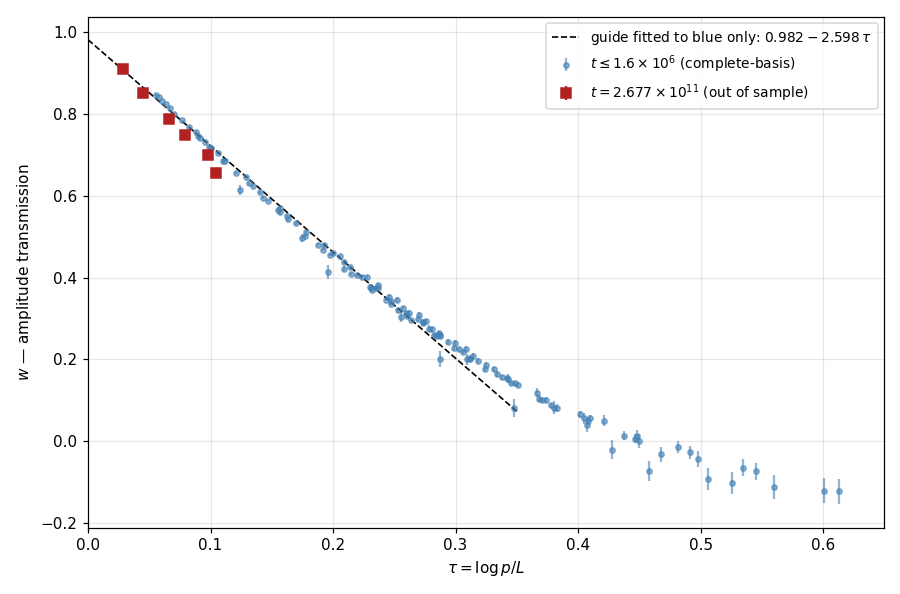
\includegraphics[width=0.82\textwidth]{fig_tau_en.png}
\caption{The amplitude-channel transmission $w$ against
$\tau = \log p / L$, complete-basis convention. Blue: the 132
measurements at $t \le 1.6\times10^6$. Red: the six out-of-sample
measurements at $t = 2.677\times10^{11}$. Dashed: the linear guide
fitted only to the blue points.}
\label{fig:tau}
\end{figure}

The results, with the small-height laws quoted as predictions:
\begin{itemize}
\item \emph{$\tau$-law for $w$}: the complete-basis linear guide
$0.982 - 2.598\,\tau$, fitted only to small heights ($\tau < 0.30$),
predicts the six measured $w_p$ at $L=24.475$ to within
$0.001$--$0.055$; e.g.\ $w_2 = 0.9097 \pm 0.0035$ against the guide
value $0.9086$. The residuals grow mildly with $\tau$ (the true curve
is not exactly linear), but the collapse variable survives the jump.
\item \emph{Sum rule}: $|u_q| = 0.99$--$1.07$ for eleven of the twelve
frequencies tested (previous convention; uncertainties $\pm 0.02$ at
$q=2$ growing to $\pm 0.2$ at the largest $q$); the twelfth, $q = 49$,
gives $1.18$, $0.9\sigma$ from unity.
\item \emph{Role-crossover}: at this $L$ the crossover law places
$Q_{\mathrm{peak}} = e^{0.40 L} \approx 2\times10^4$, so the entire
accessible range $Q \le 300$ ($\tau \le 0.233$) should lie \emph{before}
the peak: $r^*(Q)$ should rise without declining. It does
($0.901 \to 0.959$), in contrast to the peak-and-decline seen at
$L = 12.45$ over the same $Q$ range --- a successful qualitative
out-of-sample prediction.
\item \emph{Intrinsic variance}: the linear extension of
$V_{\mathrm{res}}(L)$ predicts $0.617$ at this height; the measured value
is $0.650$, high by $5\%$ in the direction expected from the (necessarily)
incomplete stripping at this $L$.
\item \emph{Effective dimension}: the $N_{\mathrm{eff}}$ test is
\emph{inconclusive} here, neither confirming nor refuting the constant
shifts: $r_{\mathrm{CUE}}(N)$ flattens at large $N$
($\mathrm{d}r/\mathrm{d}N \approx 0.008$), so with $10^4$ gaps the
uncertainty on $N_{\mathrm{eff}}$ is $\approx 0.8$. The raw deficit
$r_\zeta - r_{\mathrm{CUE}}(N{=}L) = -0.014 \pm 0.006$ is consistent with
the small-height value $-0.019$.
\end{itemize}

\subsection*{Second-order lines}
Prompted by an adversarial re-analysis of our own pipeline, we searched
the amplitude series for content at \emph{composite} frequencies
$\log(pq)$ and $\log(p/q)$, $p, q \in \{2,3,5,7\}$ --- frequencies at
which the von Mangoldt function vanishes, so the linear explicit formula
predicts nothing. The product lines are present at the few$\times10^{-3}$
level: individually $2$--$5\sigma$ per window, but coherently
\emph{cosine-locked with negative sign} in all $13$ significant
(window, line) measurements across three windows --- a sign pattern with
chance probability $\sim 2^{-13}$. The difference lines are much weaker
or absent. This asymmetry refutes the simplest mechanism (a quadratic
rectification of the real wave sum, which would feed sums and differences
equally) and suggests the second-order response is \emph{analytic} in the
wave phases, retaining $e^{i(\theta_p+\theta_q)}$ without the conjugate
cross-terms. The total log-variance carried by these lines is
$\sim 10^{-4}$, negligible for $V_{\mathrm{res}}$; their interest is
structural, not budgetary. The sampling-grid coupling identified in this
revision is a natural candidate mechanism for sign-coherent composite
lines, and their re-examination under the complete basis is pending.

\section{The gap channel at the $10^{21}$-st and $10^{22}$-nd zeros}

At heights $t \sim 10^{20}$ the Riemann--Siegel main sum has $\sim 10^{10}$
terms and amplitude computation is out of reach. The zero-displacement
channel, however, requires only zero \emph{locations}. Using Odlyzko's
tables of the $10^4$ zeros following the $10^{21}$-st and $10^{22}$-nd
zeros \cite{OdlyzkoTables} ($L = 44.58$ and $46.83$; stated accuracy
$10^{-6}$; wave phases anchored at the tables' integer base offsets), we
regressed the unfolded gap sequence on the six prime waves. All twelve
(prime, height) coefficients are detected at $3$--$5\sigma$ and agree with
the small-$\tau$ guide $v = 2.014\,\tau$ --- fitted only to the
$t \le 2.7\times10^{11}$ data --- within their uncertainties; the most
distant point gives $v_2 = 0.0297 \pm 0.0095$ against the predicted
$0.0298$. (Both sides of this comparison use the previous convention ---
an internally consistent check; the complete-basis re-measurement at
these extreme heights, where the basis cap binds, is pending, the
primary-height revision shifting $|v|$ downward by $10$--$18\%$.) Placebo frequencies sit at the noise floor
(Figure~\ref{fig:v}).

The gap-channel $\tau$-law is thereby verified over \emph{eighteen orders
of magnitude} in height: re-measuring the channel on the low-height
dataset of \cite{companion} extends it down to $t \approx 1.1\times10^3$,
and the present tables carry it to $1.4\times10^{21}$. The low windows
also reach $\tau$ up to $0.46$, where the $v$-curve is seen to bend away
from its linear onset and saturate near $0.55$--$0.60$ --- in the same
region as the role-crossover $\tau^* \approx 0.40$ of the exhaustion
analysis, as one would expect if absorption is nearly complete there. The previously quoted linear onset $v \approx 2\tau$ was a
previous-convention value; the complete-basis primary windows prefer a
shallower onset (slope $1.6$--$1.7$ for $\tau < 0.2$, depending on
whether the fit is anchored at the origin), whose exact
small-$\tau$ behavior --- and the extreme-height comparison above ---
will be settled together in the pending re-measurement.

\begin{figure}[ht]
\centering
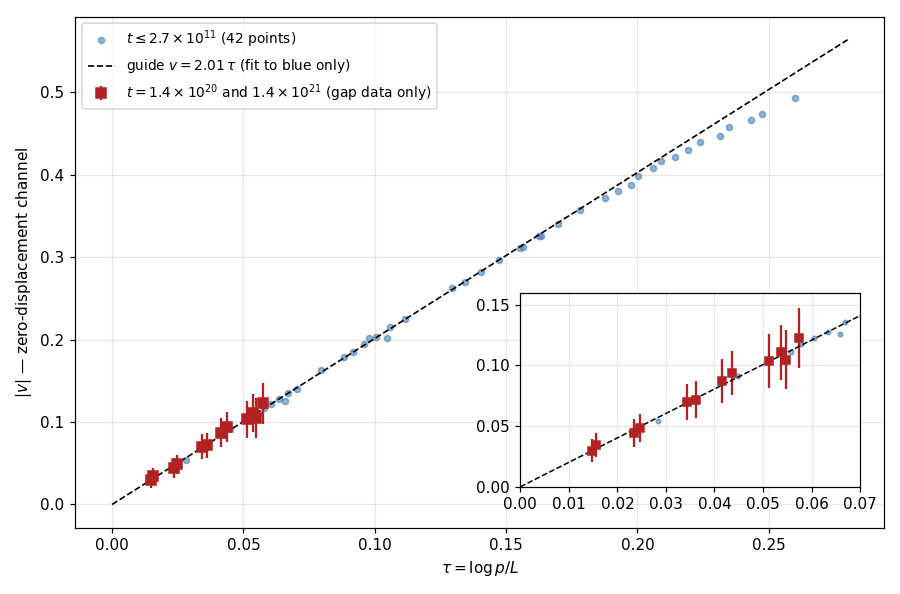
\includegraphics[width=0.82\textwidth]{fig_v_en.png}
\caption{The zero-displacement transmission $|v|$ against
$\tau = \log p/L$ (previous convention on both axes of the comparison;
complete-basis re-measurement pending). Blue: measurements at
$t \le 2.7\times10^{11}$. Red: the twelve gap-only measurements at
$t = 1.4\times10^{20}$ and $1.4\times10^{21}$. Dashed: the linear guide
fitted only to the blue points. Inset: the small-$\tau$ region.}
\label{fig:v}
\end{figure}

\section{What this says, and what it does not}

At single-gap scale, the ``randomness'' of $|Z|$ between zeros is, to two
thirds or more, deterministic prime signal carried at full
explicit-formula weight; the celebrated CUE resemblance of the
gap--amplitude law is a single-statistic compensation, not a model
equivalence. None of this bears directly on the Riemann Hypothesis, and
none of it is a closed-form claim: the two candidate closed forms this
project produced at smaller heights were both refuted by larger-$T$ tests
and are recorded as such in the project log. What survives are measured
curves --- $w(\tau)$, $v(\tau)$, the sum rule with a common
transmission factor, the crossover $\tau^*$ with the sign crossing at
$0.447$, and the basis-insensitive stripped core $r^* = 0.977$ --- each
stable across a factor $13$ in height within the primary windows (and
far beyond in the out-of-sample tests), each protected by placebo
controls, and now each quoted in a convention audited against a
ground-truth synthetic test.

Open problems: (1) derive $w(\tau)$ and $v(\tau)$ --- equivalently the
partition of the unit explicit-formula weight --- from a screening theory
of the zero gas; (2) explain $\tau^* \approx 0.40$; (3) determine the
nature of $V_{\mathrm{res}}$, whose CUE-like growth rate at reduced
magnitude suggests a small genuinely-random component of the zero gas;
(4) determine how much of the previously reported $u_q$ drift and
fixed-$\tau$ per-prime splitting survives the corrected convention ---
the sampling-grid coupling is the prime suspect; (5) pin the residual
absorption $1 - w(0)$, now consistent with $0$--$0.06$, via the
five-model re-extrapolation;
(6) recover the discriminating power of the $N_{\mathrm{eff}}$ test at
large heights, which needs $\gtrsim 10^5$ consecutive zeros there
(e.g.\ from the Platt/LMFDB datasets); (7) explain the sum-only,
sign-coherent structure of the second-order lines.

\section*{Reproducibility}

All measurements are scripts 27--84 in
\url{https://github.com/azizran/deney} (directory \texttt{qm\_riemann/}),
runnable from the stored gap--maximum datasets; the dated research log in
the same directory records the failed intermediate models (independent-phase
and common-phase generative attempts) alongside the results reported here.

\section*{Acknowledgements}

Computational assistance, literature search and drafting: Claude
(Anthropic). Errors are the author's.

\begin{thebibliography}{9}

\bibitem{Berry88} M.~V.~Berry, \emph{Semiclassical formula for the number
variance of the Riemann zeros}, Nonlinearity \textbf{1} (1988), 399--407.

\bibitem{CG85} J.~B.~Conrey, A.~Ghosh, \emph{A mean value theorem for the
Riemann zeta-function at its relative extrema on the critical line},
J. London Math. Soc. (2) \textbf{32} (1985), 193--202.

\bibitem{FZ05} K.~Ford, A.~Zaharescu, \emph{On the distribution of
imaginary parts of zeros of the Riemann zeta function}, J. reine angew.
Math. \textbf{579} (2005), 145--158.

\bibitem{FSZ09} K.~Ford, K.~Soundararajan, A.~Zaharescu, \emph{On the
distribution of imaginary parts of zeros of the Riemann zeta function,
II}, Math. Ann. \textbf{343} (2009), 487--505.

\bibitem{GHK07} S.~M.~Gonek, C.~P.~Hughes, J.~P.~Keating, \emph{A hybrid
Euler--Hadamard product for the Riemann zeta function}, Duke Math. J.
\textbf{136} (2007), 507--549.

\bibitem{HLPC24} C.~Hughes, S.~Lugmayer, A.~Pearce-Crump, \emph{The second
moment of the Riemann zeta function at its local extrema},
arXiv:2411.05573 (2024); J. London Math. Soc. (2) (2025), e70250.

\bibitem{KS00} J.~P.~Keating, N.~C.~Snaith, \emph{Random matrix theory and
$\zeta(1/2+it)$}, Comm. Math. Phys. \textbf{214} (2000), 57--89.

\bibitem{OdlyzkoTables} A.~M.~Odlyzko, \emph{Tables of zeros of the
Riemann zeta function},
\url{https://www-users.cse.umn.edu/~odlyzko/zeta_tables/}.

\bibitem{companion} U.~Sezen, \emph{The joint law of zero gaps and local
maxima of Hardy's $Z$-function: a numerical study and a CUE
effective-dimension anomaly}, draft (2026), same repository.

\end{thebibliography}

\end{document}
